% blunt_wedge.tex

\newpage
\section{Hypersonic flow of ideal air over a blunt wedge}
\label{blunt-wedge-sec}
%
This example is a partial solution to the CFD exercise for
the MECH4470 class in 2004.
Because the original specification was given in nondimensional form,
an arbitrary 10\,mm nose radius has been selected for the
inviscid simulation.
This is also a reasonable size for a possible wind tunnel experiment.
The free-stream condition was specified as having a Mach number of 5
and the gas was specified as ideal air.
Choosing particular values of $p_{\infty} = 100$\,kPa, $T_{\infty} = 100$\,K, 
lead to a free-stream velocity of $u_{\infty} = 1002$\,m/s and 
a dynamic pressure of $q_{\infty} = 1.75$\,MPa.

\begin{figure}[htbp]
\begin{center}
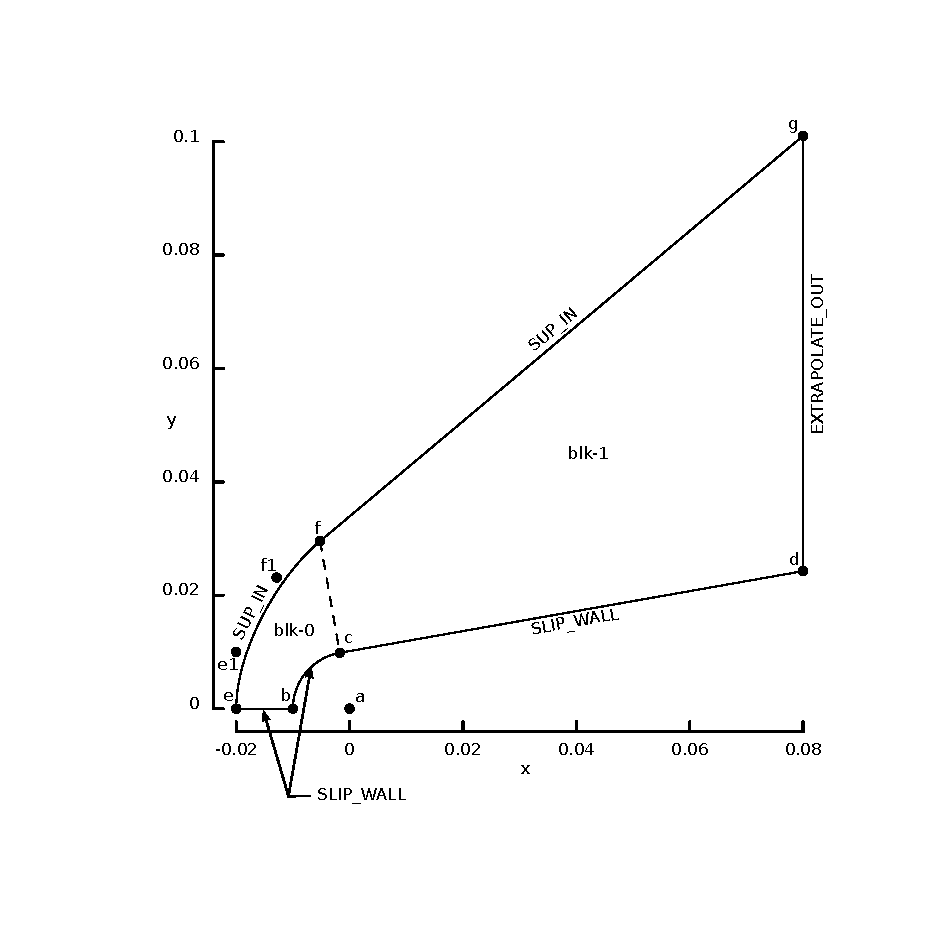
\includegraphics[width=10cm,viewport=77 67 398 398,clip=true]{../2D/blunt-wedge/bw-layout.pdf}
\end{center}
\caption{Schematic diagram of the geometry for the blunted 10 degree wedge.}
\label{bw-geometry-fig}
\end{figure}

\begin{figure}[htbp]
\begin{center}
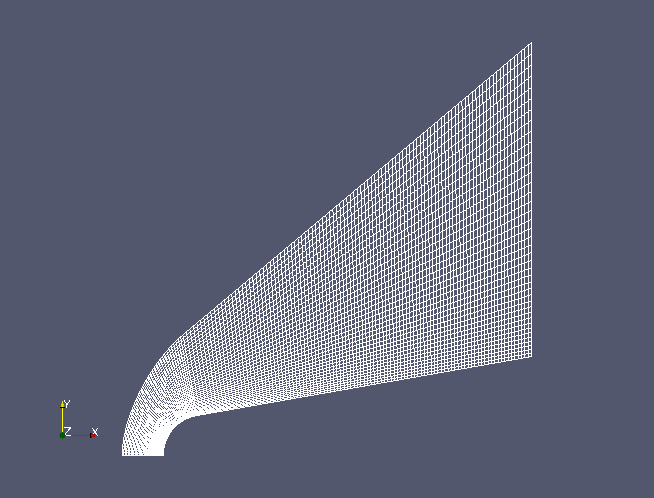
\includegraphics[width=0.8\textwidth]{../2D/blunt-wedge/bw-mesh.png}
\end{center}
\caption{Mesh for the blunt wedge exercise.}
\label{bw-mesh-fig}
\end{figure}

\medskip
The simulation is started with low-pressure conditions throughout the flow
domain and free-stream conditions applied to the inflow boundary
(the west boundary of blk-0 and the north boundary of blk-1).
The flow data is allowed to evolve until $t_{final} = 399\,\mu$s,
which corresponds to a particle of the free-stream travelling 40 nose radii.
The axial force (shown in Fig.\ref{bw-xforce-fig}) is seen to settle to 
a value of 28590\,N in that time.
This corresponds to a drag coefficient of 0.674.

\begin{figure}[htbp]
\begin{center}
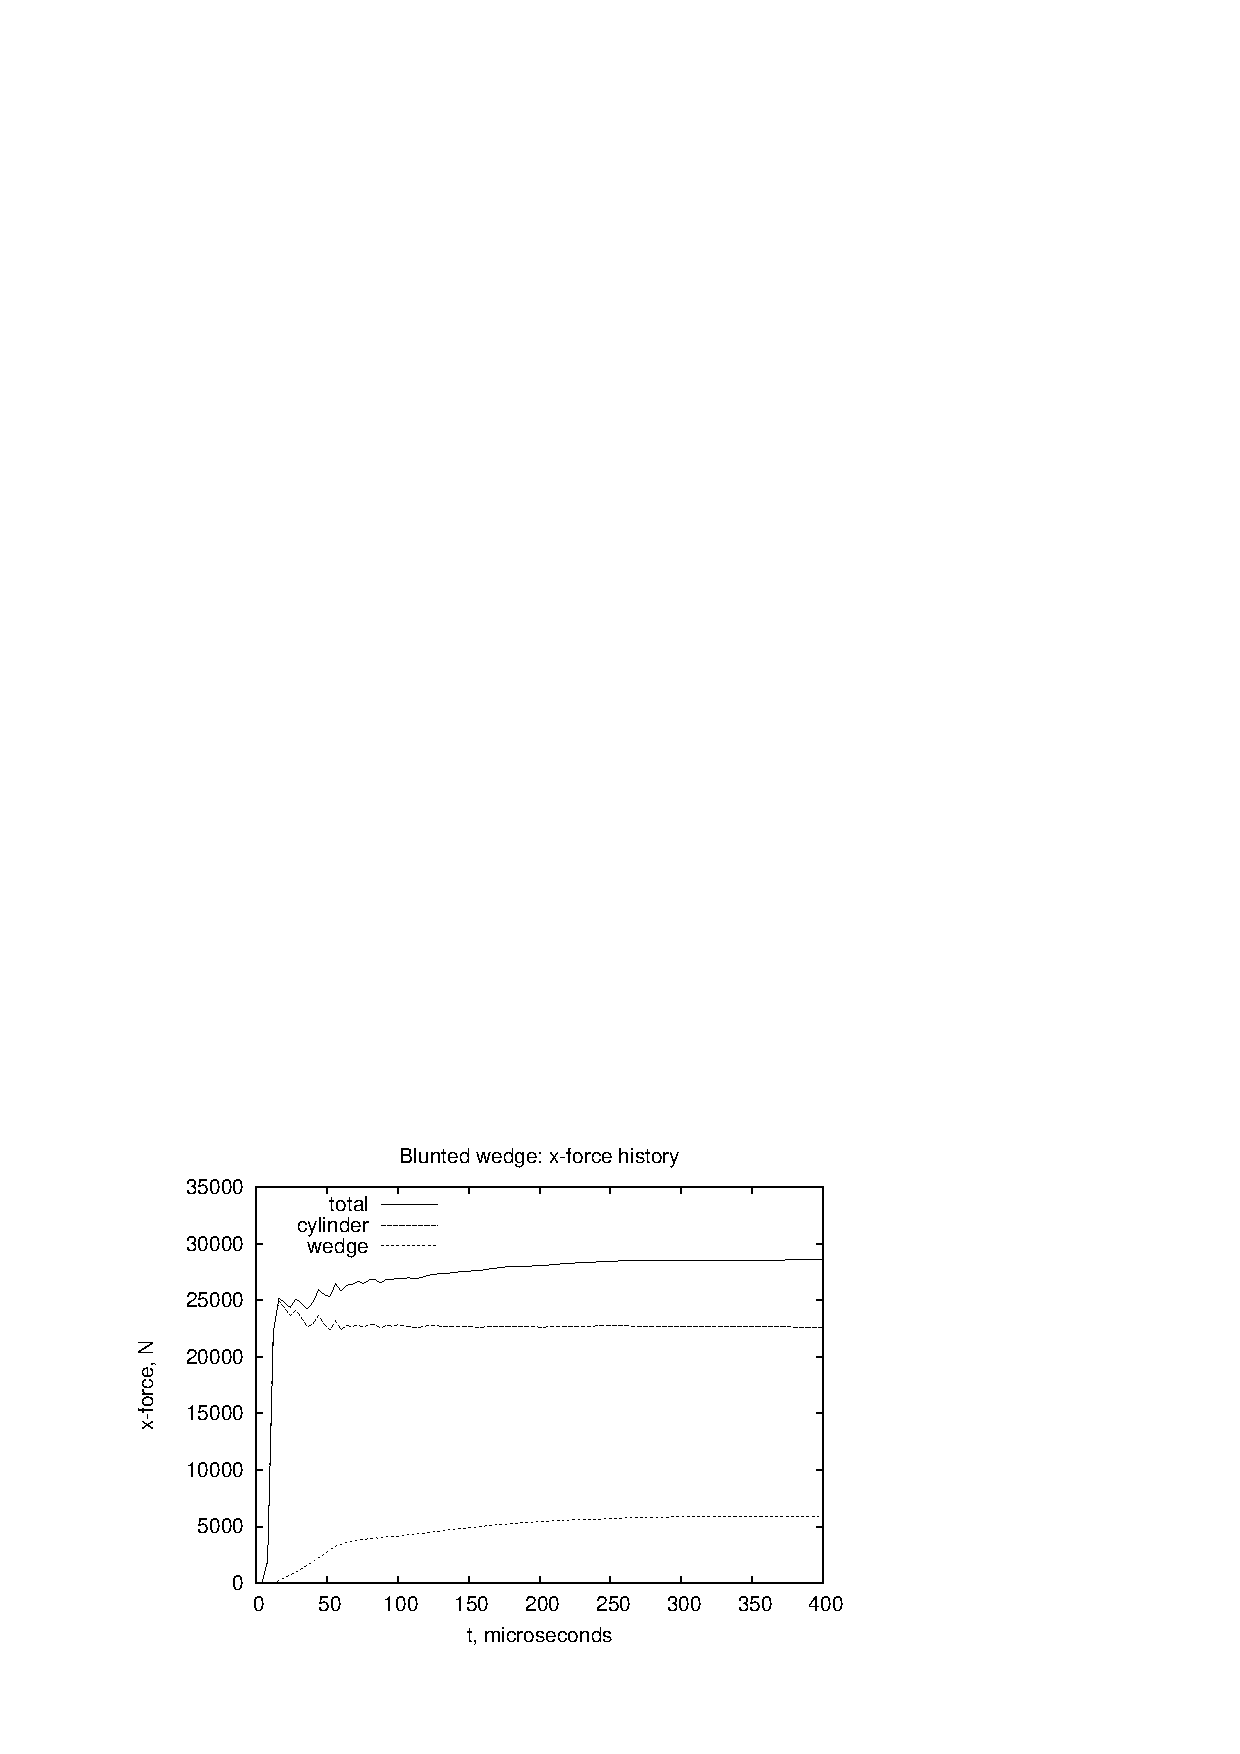
\includegraphics[width=12cm,viewport=66 52 404 292,clip=true]{../2D/blunt-wedge/bw_xforce.pdf}
\end{center}
\caption{History of the axial forces for the blunt-wedge exercise.}
\label{bw-xforce-fig}
\end{figure}

\begin{figure}[htbp]
\begin{center}
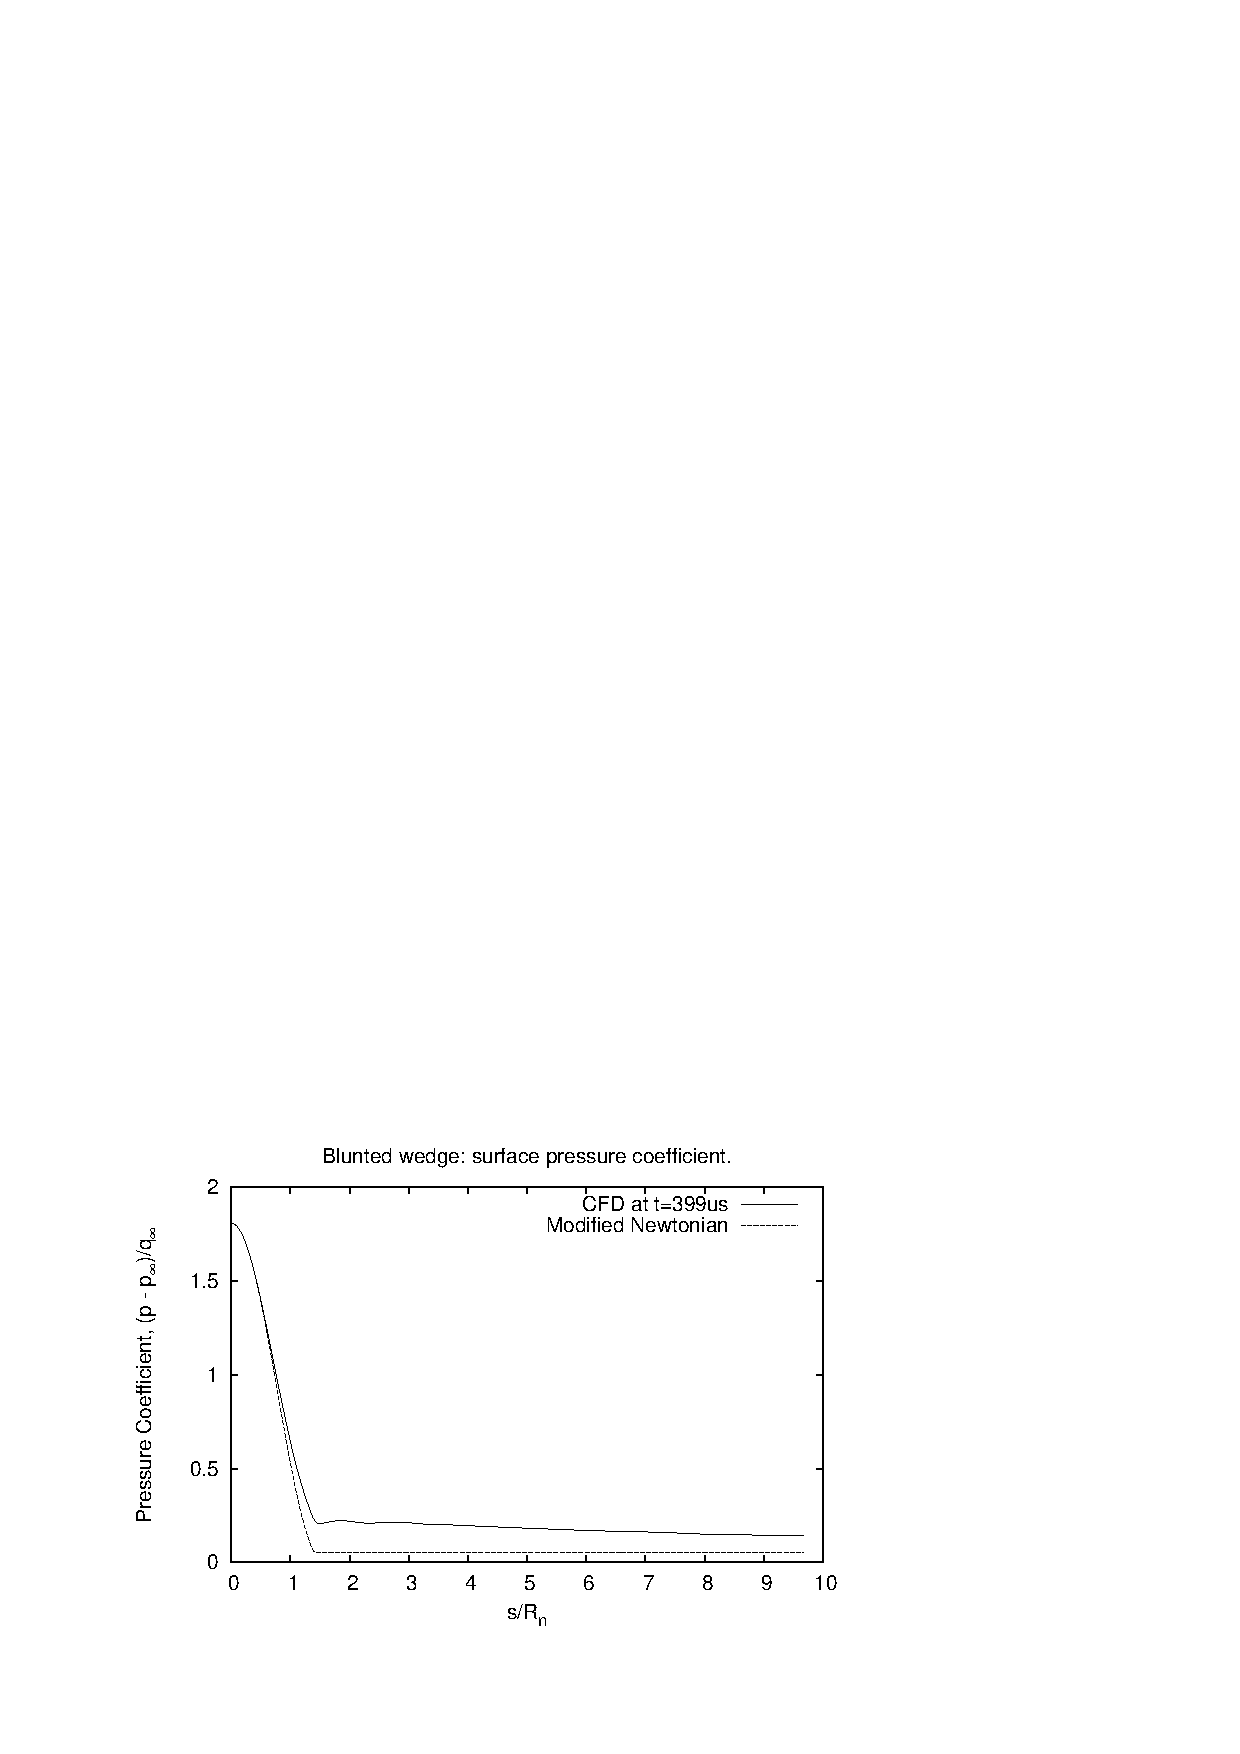
\includegraphics[width=12cm,viewport=64 61 401 291,clip=true]{../2D/blunt-wedge/bw_surface_pressure.pdf}
\end{center}
\caption{Surface pressure coefficient data for the blunt-wedge exercise.}
\label{bw-surface-pressure-fig}
\end{figure}

\medskip
The surface pressure (shown normalised in Fig.~\ref{bw-surface-pressure-fig})
has been extracted from the solution file by \texttt{e3post.py} by selecting the
east-most line of cells of the first block and the south-most line of cells
of the second block.
The selected data is filtered by an Awk script to produce the normalised data
(and the Newtonian reference data) as plotted.

\begin{figure}[htbp]
\begin{center}
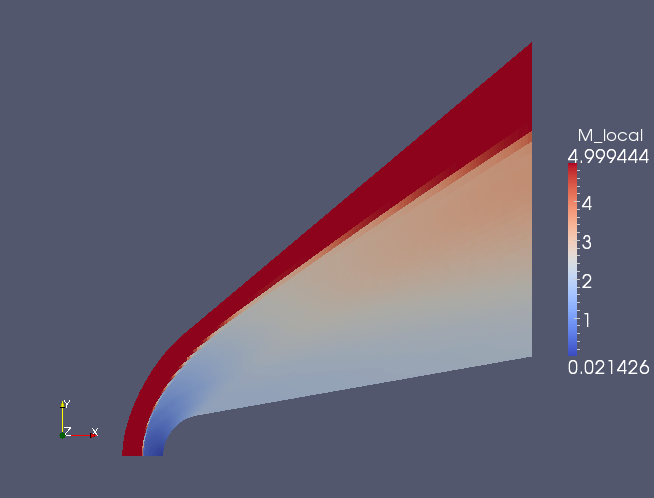
\includegraphics[width=0.8\textwidth]{../2D/blunt-wedge/bw-Mach-field.png}
\end{center}
\caption{Mach number data for the blunt-wedge exercise.}
\label{bw-Mach-fig}
\end{figure}

\newpage

\subsection{Input script (.py)}\index{xforce\_list!example of use}
\topbar
\lstinputlisting[language={}]{../2D/blunt-wedge/bw.py}
\bottombar

\newpage
\subsection{Shell scripts}
\label{bw-sh-files}
\topbar
\lstinputlisting[language={}]{../2D/blunt-wedge/bw_prep.sh}
\bottombar

\noindent
\topbar
\lstinputlisting[language={}]{../2D/blunt-wedge/bw_run.sh}
\bottombar

\noindent
\topbar
\lstinputlisting[language={}]{../2D/blunt-wedge/bw_post.sh}
\bottombar

\newpage
\subsection{Notes}
\begin{itemize}
\item This simulation reaches a final time of 399\,$\mu$s.
      For \texttt{mbcns2} on an Intel Pentium-M 1.73\,Ghz system, this took 6\,min, 39\,s of CPU time
      for 3722 steps.
      However, for \texttt{Eilmer3} on an Intel E2140 1.6Ghz system it now takes 15\,m, 23\,s
      for 3759 steps.
\item Selection of the \texttt{e3shared.log} file showing some x-force data
      as written during the simulation.
      Pressure and viscous forces are written separately.
      Note that the lines are written with several items separated by spaces and the
      format is mostly self-documenting.
      The only extra bit of information is that BNDY values are 0, 1, 2 and 3 for
      boundaries NORTH, EAST, SOUTH and WEST, respectively.
\footnotesize
\begin{verbatim}
Step=    420 t= 2.747e-05 dt= 9.100e-08 WC=102.0 WCtFT=991.8 WCtMS=1112.3
CFL_min = 1.862345e-03, CFL_max = 4.958796e-01, dt_allow = 9.100331e-08
Smallest CFL_max so far = 3.381457e-02 at t = 1.000000e-07
 dt[0]=9.100331e-08 dt[1]=1.500771e-07
There are 2 active blocks.
RESIDUAL mass block 0 max: 4.899825e-02 at (-0.00280173,0.0146712,0)
RESIDUAL energy block 0 max: 5.025321e-02 at (-0.00280173,0.0146712,0)
RESIDUAL mass block 1 max: 1.656031e-01 at (0.0254165,0.0185377,0)
RESIDUAL energy block 1 max: 4.834703e-01 at (0.0262722,0.0181336,0)
RESIDUAL mass global max: 1.656031e-01 step 420 time 2.74667e-05
RESIDUAL energy global max: 4.834703e-01 step 420 time 2.74667e-05
XFORCE: TIME 2.801336e-05 BLOCK 0 BNDY 1 FX_P 2.415181e+04 FX_V 2.204480e+00 
XFORCE: TIME 2.801336e-05 BLOCK 1 BNDY 2 FX_P 9.973561e+02 FX_V 9.133770e+00 
\end{verbatim}
\normalsize

\item Awk filter for extracting the x-force data from the simulation log file.
      Note that there are two pattern-action rules, one for each block.
      \lstinputlisting[language={}]{../2D/blunt-wedge/xforce.awk}
\item Awk filter for normalising the surface pressure data.
      \lstinputlisting[language={}]{../2D/blunt-wedge/surface_pressure.awk}
\end{itemize}
